\newpage
\section{Reproducible Test Environment}

The scope of this thesis is confined to the AI-NSAK reconnaissance scenario, including the design and implementation of corresponding drills.

To ensure a controlled and safe evaluation of the implementation, a simulated test environment is established. This approach prevents unintended interference with production systems during the development and testing phases.

Building upon a preceding project, a simplified network topology consisting of a client (Alice) and a server (Bob) is utilized to emulate and analyze a Layer 2 man-in-the-middle (MITM) scenario.
\todo{Insert reference to Project 2}
While Docker or Podman provides a general-purpose containerization platform, they lack the support for modeling network topologies. In contrast, ContainerLab\cite[]{containerlab} builds upon Docker and optimize its functionalities for networking purposes. 

A primary advantages of ContainerLab are:
\begin{itemize}
	\item It`s ability to create a reproducible containerized network topology based on a simple configuration file
	\item Support multiple interfaces nodes which closely resemble real-world network devices. (in comparison Docker typically operate with a single network interface)
	\item The rapid creation, extension and teardown of complete network environments, ensure that each experiment starts from a clean and controlled state.
\end{itemize}
In summary, while OCI container serves as the underlying container engine, ContainerLab provides a higher-level network simulation.

The following listing shows an excerpt of the Containerlab topology.yaml file as a segmented enterprise network consisting of WAN, DMZ, and LAN zones. The configuration includes a firewall node that implements traffic filtering policies, as well as multiple hosts representing typical enterprise assets.

\begin{yamlcode}
topology:
 nodes:
  firewall:
  kind: linux
  image: alpine:3.19
  cap-add:
   - NET\_ADMIN
  sysctls:
   net.ipv4.ipforward: 1
 
  dmz-server:
   kind: linux
   
  ctrl-server:
   kind: linux
 
 links:
  # WAN segment (WAN 10.0.1.0/24)
  - endpoints: [ "firewall:eth1", "wan-br:fw1" ]
  - endpoints: [ "external:eth1" , "wan-br:ext" ]
  # DMZ segment (172.16.1.0/24)
  - endpoints: [ "firewall:eth2", "dmz-br:fw2" ]
  - endpoints: [ "dmz-server:eth1", "dmz-br:dmz-serv" ]
  # LAN segment (192.168.10.0/24)
  - endpoints: [ "firewall:eth3", "lan-br:fw3" ]
  - endpoints: [ "ctrl-server:eth1", "lan-br:ctrl" ]
  - endpoints: [ "alice:eth1", "lan-br:A" ]
  - endpoints: [ "bob:eth1", "lan-br:B" ]
  - endpoints: [ "printer:eth1", "lan-br:print" ]
\end{yamlcode}
\captionof{listing}{Excerpt of the Containerlab topology definition}
\label{lst:containerlab}

\subsection{Network Topology}

The network topology shown in Figure~\ref{fig:virtual-environments} illustrates the IP addressing scheme and the interconnections between the individual components. The \textit{external} node represents the perspective of an outside attacker interacting with the network from the WAN. The \textit{nsak} container can be deployed across different network segments, enabling the simulation of various attacker positions and reconnaissance scenarios.

The 
\begin{figure}[H]
	\centering
	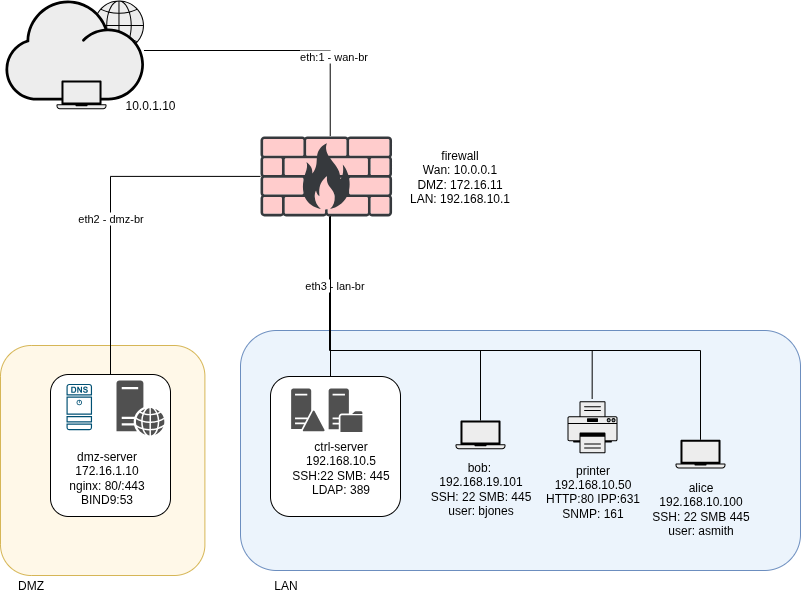
\includegraphics[width=0.7\linewidth]{../assets/diagrams/virtual-environments/virtual-environments.drawio}
	\caption{}
	\label{fig:virtual-environments}
\end{figure}

\subsection{Services}
